% !TeX encoding = UTF-8
% !TeX program = pdflatex
% !BIB program = bibtex

%%% Um einen Artikel auf deutsch zu schreiben, genügt es die Klasse ohne
%%% Parameter zu laden.
\documentclass[]{lni}
\usepackage{float}
\usepackage[normalem]{ulem}

\newcommand{\quoteStyle}{alphabetic}
\usepackage[
	backend=biber,		% recommended. Alternative: bibtex
	bibwarn=true,
	bibencoding=utf8,	         % If .bib file is encoded with utf8, otherwise ascii
	sortlocale=de,
	style=\quoteStyle
]{biblatex}
\addbibresource{bibliographie.bib}

\graphicspath{{bilder/}}

%%% To write an article in English, please use the option ``english'' in order
%%% to get the correct hyphenation patterns and terms.
%%% \documentclass[english]{class}
%%
\begin{document}
%%% Mehrere Autoren werden durch \and voneinander getrennt.
%%% Die Fußnote enthält die Adresse sowie eine E-Mail-Adresse.
%%% Das optionale Argument (sofern angegeben) wird für die Kopfzeile verwendet.
\title[Everything-as-a-Service]{XaaS: Künstliche Intelligenz im Trend von Everything-as-a-Service}
%%%\subtitle{Untertitel / Subtitle} % if needed
\author[Niklas Arnold \and Luca Negron-Martinez]
{Niklas Arnold\footnote{DHBW Stuttgart Campus Horb, Informatik, Florianstraße 15, 72160 Horb am Neckar, Deutschland \email{i20002@hb.dhbw-stuttgart.de}} \and
Luca Negron-Martinez\footnote{DHBW Stuttgart Campus Horb, Informatik, Florianstraße 15, 72160 Horb am Neckar, Deutschland
\email{i20024@hb.dhbw-stuttgart.de}}}
\startpage{1} % Beginn der Seitenzählung für diesen Beitrag / Start page
\editor{DHBW Stuttgart Campus Horb} % Names of Editors
\booktitle{Advanced Software Engineering} % Name of book title
\yearofpublication{2022}
%%%\lnidoi{18.18420/provided-by-editor-02} % if known
\maketitle

\begin{abstract}
Diese Seminararbeit widmet sich dem Thema Everything-as-a-Service, oder kurz XaaS. Hierbei werden kurz die drei Hauptkomponenten davon erläutert und die Frage, was Xaas überhaupt ist geklärt. Danach wird dann der Fokus auf den Bereich von AIaaS, also der künstlichen Intelligenz als Service gelegt. Dabei werden verschiedene Einsatzbereiche und Anwendungsmöglichkeiten aufgezeigt und welche Anbieter welche Systeme zur Verfügung stellen. Diese Darstellung wird mit Hilfe einer Marktanalyse realisiert. Bei AIaaS gibt es viele Vor-, jedoch auch einige Nachteile bzw. Risiken. Pro- und Contra-Argumenten werden mit einer Argumentation gegenübergestellt und analysiert. 
Zusammenfassend wird dargestellt, warum AIaaS immer weiter verbreitet ist und wie sich der Nutzen in der Zukunft weiterentwickeln könnte.
\end{abstract}

\begin{keywords}
XaaS \and AIaaS \and Künstliche Intelligenz
\end{keywords}

%%% Beginn des Artikeltexts
\section{Einleitung}
\subsection{Motivation}
Unsere Welt befindet sich in einem andauernden Umbruch. Immer mehr befindet sich in einem stetigen Wandel. Alles wird schneller und kurzlebiger. So ist es auch in der Informatik, speziell in der Softwareentwicklung bzw. der Bereitstellung von Software. Die Anforderungen an ein heutiges System sind vor allem Flexibilität und Agilität. Hier kommt die Idee von XaaS ins Spiel. Unter XaaS versteht das Prinzip von Everything-as-a-Service. Unter diesem Ansatz versteht man hauptsächlich Dienstleistungen rund um Infrastruktur (IaaS), Software (SaaS) und Plattformen (PaaS) als einen Service zu beziehen. Erweitert reicht XaaS aber auch bis hin zum Einsetzen von künstlicher Intelligenz als Service (AIaaS). Bei einer solchen Umstellung auf serviceorientierte Betriebsmodelle kann der Verwaltungsaufwand erheblich sinken, da man sich nicht mehr um die Wartung und Instandhaltung der genutzten Dienste kümmern muss. Außerdem können durch ein solches Modell die Anwendungen und Systeme nach Bedarf skaliert werden. Dadurch entfallen die Kosten für die Altsysteme und es entstehen ausschließlich neue Kosten für die in Anspruch genommenen Leistungen. \\
\subsection{Fragestellung}
Immer mehr Anwendungen basieren auf einer Künstlichen Intelligenz. Ob es diverse Bilderkennungstools, Chatbots oder maschinelle Übersetzer sind, immer mehr setzt man auf die neuronalen Netze.
Bei einer genaueren Betrachtung von XaaS ergeben sich mehrere Fragen, welche es zu beantworten gilt. Zum einen, was ist Everything-as-a-Service? Darunter zählt was man unter XaaS versteht, sowie in welche Unterpunkte man den Begriff untergliedern kann. Der Fokus soll dabei auf AIaaS, also Artificial Intelligence-as-a-Service (Künstliche Intelligenz als Service), liegen. Hierbei wird auf den Nutzen, die möglichen Anwendungsbereiche, sowie die Vor- und Nachteile eingegangen, um abwägen zu können, welche Faktoren AIaaS bzw. XaaS allgemein begünstigen und weshalb sie von immer mehr Unternehmen eingesetzt werden. Außerdem soll analysiert werden, auf welche Serviceanbieter hier in der Regel zurückgegriffen wird, welche Funktionen und Tools sie anbieten und wie dabei das jeweilige Preismodell aufgebaut ist. \\
\section{Everything-as-a-Service}
\subsection{Was ist XaaS?}
Everything-as-a-Service, auch als XaaS bekannt, ist ein Begriff, der die Bereitstellung einer breiten Palette von Diensten über das Internet beschreibt. Diese Dienste können über herkömmliche webbasierte Anwendungen oder, was häufiger gemeint ist, über modernere cloudbasierte Plattformen bereitgestellt werden. XaaS kann alles umfassen, von Speicher- und Sicherungsdiensten über Software und Anwendungen bis hin zu Infrastruktur- und Plattformdiensten. \cite[vgl.][986f.]{Kollmann.2020} Im Grunde genommen kann jeder Dienst, der über das Internet bereitgestellt werden kann, als XaaS betrachtet werden. Im weitesten Sinne ist auch Human-as-a-Service (HuaaS) miteinbegriffen, also das Nutzen von menschlicher Intelligenz über das Internet wie einen herkömmlichen Webservice. \cite[vgl.][]{CW.2022}
Der Begriff wird im Allgemeinen verwendet, um den Wechsel von herkömmlichen, vor Ort installierten Software- und Hardwarelösungen zu cloudbasierten Lösungen zu beschreiben. Mit XaaS können Unternehmen nur für die Dienste zahlen, die sie benötigen, wenn sie sie benötigen, ohne im Voraus in teure Hardware und Software investieren zu müssen. Der Begriff wird im Allgemeinen verwendet, um den Wechsel von herkömmlichen, vor Ort installierten Software- und Hardwarelösungen zu cloudbasierten Lösungen zu beschreiben. Mit XaaS wird es Unternehmen ermöglicht nur für die Dienste zu zahlen, die sie benötigen, wenn sie sie benötigen, ohne im Voraus in teure Hardware und Software investieren zu müssen. XaaS kann eine kostengünstige Möglichkeit für Unternehmen sein, die benötigten Dienste zu erhalten, ohne in die Infrastruktur zur Unterstützung dieser Dienste investieren zu müssen. Außerdem können Unternehmen dadurch flexibler werden, da sie ihre Dienste je nach Bedarf auf- oder abbauen können.

Klassisch betrachtet, spricht man bei XaaS von drei aufeinander aufbauenden Schichten. Dabei beinhaltet eine Ebene auch immer die Eigenschaften der Darunterliegenden.

\begin{figure}
  \centering
  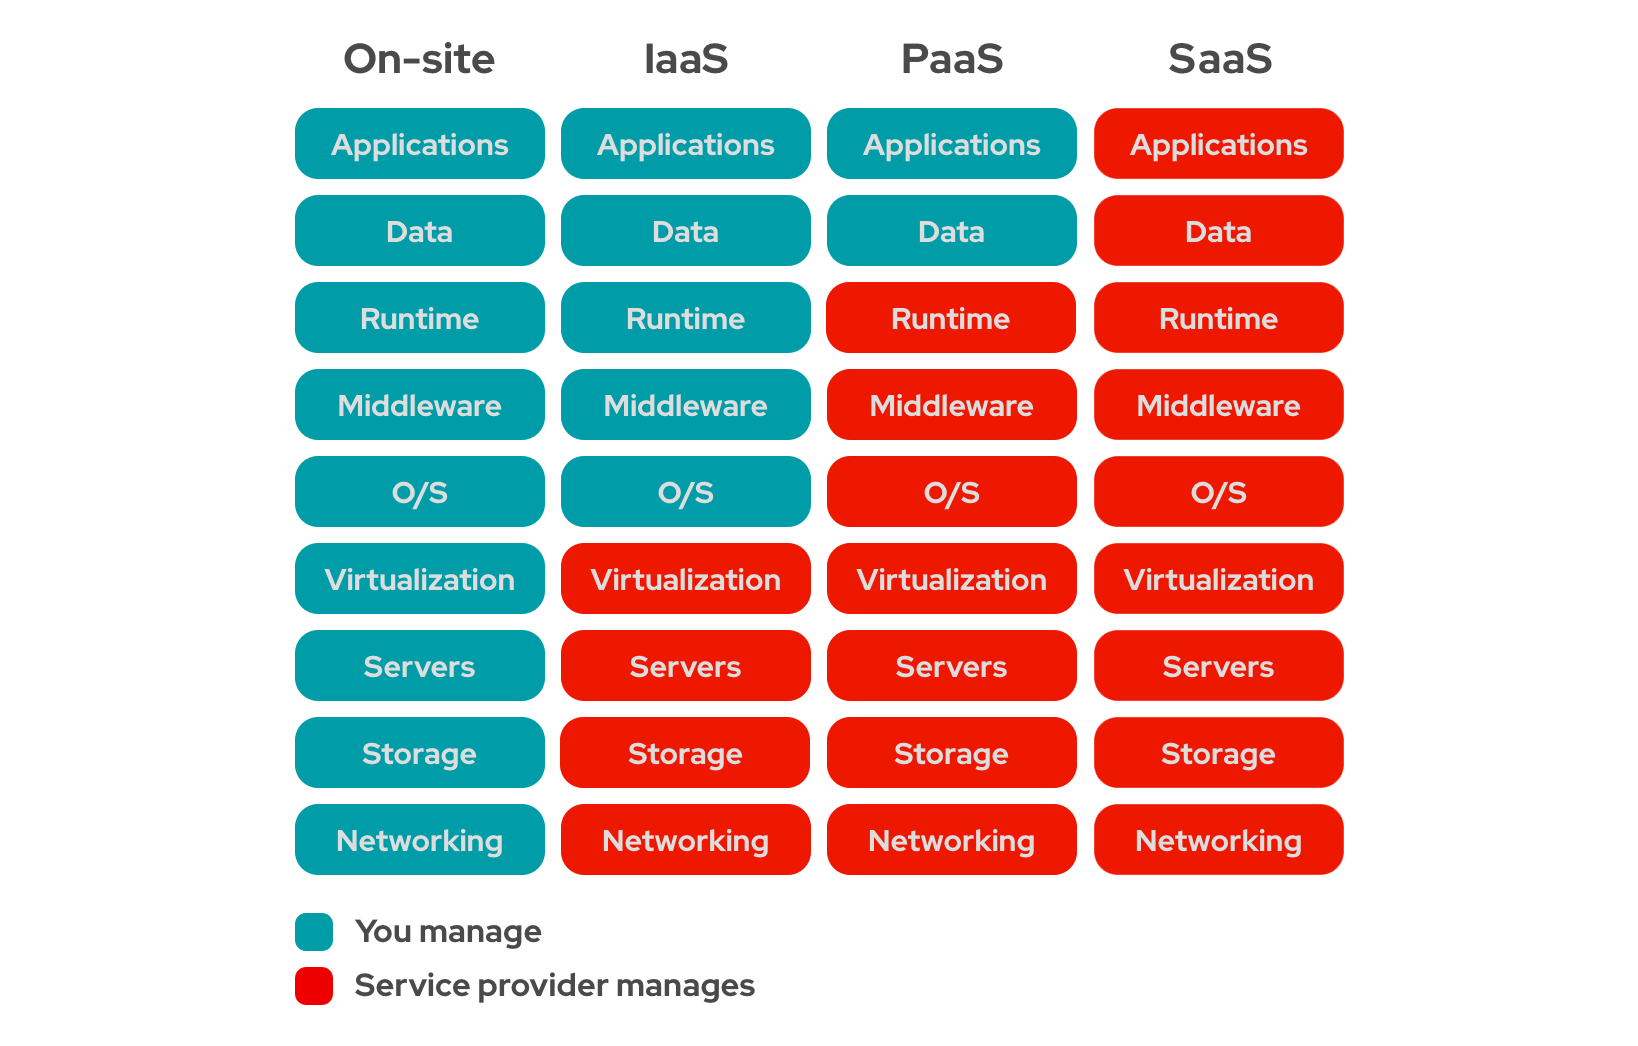
\includegraphics[width=0.9\textwidth]{bilder/xaas.png}
  \caption{Stufenartig aufgebautes Cloud Computing Modell \cite{RedHat.2022}}
  \label{fig:xaasmodell}
\end{figure}


Die drei Hauptkomponenten sind Infrastructure-, Plattform- und Software-as-a-Service. Wie in der Abbildung zu sehen ist kommen bei jeder Stufe im Gegensatz zu dem klassischen On-Site-Ansatz, bei dem jegliche Infrastruktur selbst beschafft und vor Ort gehostet wird, Services dazu, die die Service Provider verwalten und nicht mehr selbst gemanaged und gewartet werden müssen. \cite[vgl.][]{RedHat.2022}


\subsection{Infrastructure-as-a-Service (IaaS)}
Infrastructure-as-a-Service ist die unterste Ebene des dreischichtigen Servicemodells von Cloud Computing. Man versteht darunter das Modell, bei dem ein Drittanbieter eine Computerinfrastruktur als Dienst anbietet. Das heißt, bei IaaS wird das Hosting geoutsourced, wobei der IaaS-Kunde nicht der Eigentümer der Infrastruktur ist, sondern diese bei einem Provider mietet. Die IaaS-Anbieter stellen diese Ressourcen dann auf Abruf aus ihren umfangreichen, in Rechenzentren installierten Gerätepools bereit. Dieser ist dann auch für die Wartung und den Support der Hardware und Software verantwortlich, so dass sich der Kunde auf sein Kerngeschäft konzentrieren kann. Die Kunden zahlen nur für die Menge an Rechen-, Speicher- und Netzwerkressourcen, die sie nutzen, in der Regel auf einer Pay-as-you-go-Basis. Dies steht im Gegensatz zum traditionellen Modell des Kaufs und der on-premise Verwaltung von Hardware und Software, die kapitalintensiv sein können und erhebliche laufende Wartungs- und Supportkosten erfordern.

Zusammenfassend lässt sich sagen, dass IaaS ein Cloud-Computing-Modell ist, das es Unternehmen ermöglicht, das Hosting und die Wartung ihrer Hardware- und Software-Ressourcen auszulagern. Es bietet Unternehmen die Möglichkeit, Ressourcen schnell und bedarfsgerecht zu skalieren, auf die neuesten Technologien zuzugreifen, ohne in teure Hardware- und Software-Upgrades investieren zu müssen, und individuelle Lösungen für ihre spezifischen Anforderungen zu entwickeln. \cite[vgl.][31]{HuaweiTechnologies.2023} \\


\subsection{Platform-as-a-Service (PaaS)}
Die nächste Ebene im Cloud Computing Modell ist Platform-as-a-Service oder auch PaaS. PaaS-Anbieter bieten eine Umgebung an, in der Anwendungen entwickelt, ausgeführt und verwaltet werden können, ohne dabei die zugrundeliegende Infrastruktur aufbauen zu müssen. PaaS-Dienste ermöglichen es den Benutzern, über eine Internetverbindung auf eine Plattform und alle zugehörigen Dienste zuzugreifen, wodurch die Installation, Konfiguration und Verwaltung von Hardware und Software entfällt. Dies kann die Kosten senken und den Entwicklungsprozess beschleunigen. PaaS-Dienste umfassen in der Regel Betriebssysteme, Webserver, Anwendungsserver, Datenbanken, Speicherdienste und andere Dienste zur Erstellung und Bereitstellung von Anwendungen. \\
Zusammenfassend spricht man bei PaaS häufig auch von einem ,,Cloud-Betriebssystem``. PaaS kann für die schnelle Entwicklung und Bereitstellung von Webanwendungen, mobilen Anwendungen und anderen Softwareanwendungen verwendet werden, ohne dass dabei die Komplexität der Verwaltung der zugrundeliegenden Infrastruktur auf sich genommen werden muss. \cite[vgl.][31ff.]{HuaweiTechnologies.2023} \\


\subsection{Software-as-a-Sercice (SaaS)}
Auf der obersten Ebene des dreistufigen Cloud Computing Modells und somit die umfangreichste Bereitstellung von Diensten ist Software-as-a-Service oder auch SaaS. SaaS ist eine Softwarebereitstellungsmethode, bei der die gesamte Software, also inklusive Infrastruktur und Betriebssystem, auf entfernten Servern zentral gehostet wird und die Nutzer über das Internet mit einem standard Webbrowser darauf zugreifen können. SaaS-Anwendungen werden manchmal auch als webbasierte Software, On-Demand-Software oder gehostete Software bezeichnet. Mit SaaS können die Kunden von jedem Ort, zu jeder Zeit und mit jedem Gerät, das über eine Internetverbindung verfügt, auf die Software zugreifen, ohne die Software auf ihren eigenen Servern oder Geräten installieren und verwalten zu müssen. SaaS-Lösungen sind in der Regel abonnementbasiert und werden auf monatlicher oder jährlicher Basis bezahlt. \\

Diese Dienste sind sowohl für allgemeine Nutzer (Anwendungen wie Google Calendar und Gmail), als auch für Unternehmensgruppen zur Unterstützung von Gehaltsabrechnungen, Personalverwaltung, und für die Verwaltung von Kunden- und Geschäftspartnerbeziehungen. Durch diese Anwendungen wird der Zeitaufwand für die Installation und Wartung der Software reduziert und es muss auch keine Hardware, Software und spezielles IT-Personal beschafft werden. \cite[vgl.][33f.]{HuaweiTechnologies.2023} \\


\input{kapitel/begünstigung}
\newpage
\section{Artificial Intelligence-as-a-Service (AIaaS)}
Ein stark wachsender Bereich in der Digitalisierung und der Automatisierung ist die Künstliche Intelligenz. Sie kann für eine Vielzahl von Aufgaben eingesetzt werden. Sie kann zum Beispiel Analysen und Erkenntnisse liefern, Maschinen helfen Menschen zu verstehen und mit ihnen zu interagieren oder alltägliche Aufgaben automatisieren. KI wird auch im Gesundheits-, Bank- und Finanzwesen eingesetzt, um Prozesse zu automatisieren, Prognosemodelle zu erstellen und die Kundenerfahrung zu verbessern. \\
Das Erstellen und Trainieren von KI-Modellen kann allerdings sehr zeitaufwendig und gegebenenfalls auch sehr komplex sein. Außerdem benötigen KI-Anwendungen in der Regel eine hohe Rechenleistung. Somit ist es häufig in kleinen bis mittleren Unternehmen nicht gegeben, dass zum einen das notwendige KI-KnowHow und KI-Entwickler vorhanden sind und zum anderen auch die benötigte Infrastruktur nicht gegeben ist. Aus diesen Gründen gibt es auch hier eine Nachfrage nach einem cloudbasierten Produkt, mit welchem sich, ohne großes Vorwissen und Aufwand, künstliche Intelligenzen in die eigenen Anwendungen einbinden lassen. Die Lösung dafür nennt sich Artificial Intelligence-as-a-Service, oder kurz AIaaS. \cite[vgl.][441f.]{Lins.2021} \\ \\
Artificial Intelligence-as-a-Service (AIaaS), oder Künstliche Intelligenz als Service, ist ein Cloud-basierter Dienst, der es Unternehmen ermöglicht, Funktionen einer künstlichen Intelligenz in ihre Anwendungen und Systeme zu integrieren, ohne die erforderliche Infrastruktur aufbauen oder warten zu müssen. AIaaS-Lösungen können eine Reihe von Funktionen bieten, von der Verarbeitung natürlicher Sprache, Bilderkennung und maschinellem Lernen bis hin zu prädiktiven Analysen und der Automatisierung von Robotikprozessen. Sie können Unternehmen in die Lage versetzen, ihre betriebliche Effizienz zu steigern, Kosten zu senken und den Kundenservice zu verbessern.

Für den Zugriff auf die AIaaS-Lösung zahlen Unternehmen in der Regel eine Abonnementgebühr an den Anbieter, und sie können dann über eine API oder eine andere Integrationsmethode auf die KI-Funktionen zugreifen. Diese Art von Service kann Unternehmen die Ressourcen zur Verfügung stellen, die sie benötigen, um die Entwicklung von KI-Anwendungen zu beschleunigen, ohne in kostspielige Infrastruktur und Technologie investieren zu müssen. \cite[vgl.]{Cuofano.2022}
\newpage
\section{Globaler AIaaS-Markt}
Der globale Markt für Artificial Intelligence as a Service steigt immer weiter an. Die gesamte Marktgröße lag 2021 noch etwa bei 4,7 Milliarden US-Dollar, allerdings wird prognostiziert, dass der globale Markt bis 2030 auf ca. 92 Milliarden US-Dollar anwachsen könnte. Das entspräche, über einen Zeitraum von acht Jahren, einer durchschnittlichen jährlichen Wachstumsrate von 39,16 Prozent. Zu den wichtigsten Faktoren, die den Markt vorantreiben, gehören unter anderem der Bedarf und die Nachfrage an kostengünstigen KI-Lösungen von kleinen und mittelständigen Unternehmen, die Notwendigkeit die Markteinführungszeit von KI-Anwendungen zu verkürzen und der Mangel an Firmeninterner KI-Expertise. Zu den wichtigsten Akteuren auf dem Markt zählen Google LLC, IBM Corporation, Microsoft Corporation und Amazon Web Services Inc. All diese Akteure haben verschieden Konzepte, Herangehensweisen und Wachstumsstrategien wie Partnerschaften, Kooperationen und neue Produkteinführungen, um ihre Präsenz auf dem globalen Markt für künstliche Intelligenz als Dienstleistung zu etablieren und zu erweitern. Eine aussagekräftige Marktanalyse zu den jeweiligen Marktanteilen ist nicht möglich, da die Unternehmen ihre Umsatzzahlen im Bereich von AIaaS nicht einzeln veröffentlichen. Man weiß lediglich den gesamten Umsatz den sie mit künstlicher Intelligenz generieren, wovon AiaaS wohl nur ein Bruchteil davon ausmacht. \cite[vgl.][]{PR.2021} \\

\begin{figure}
  \centering
  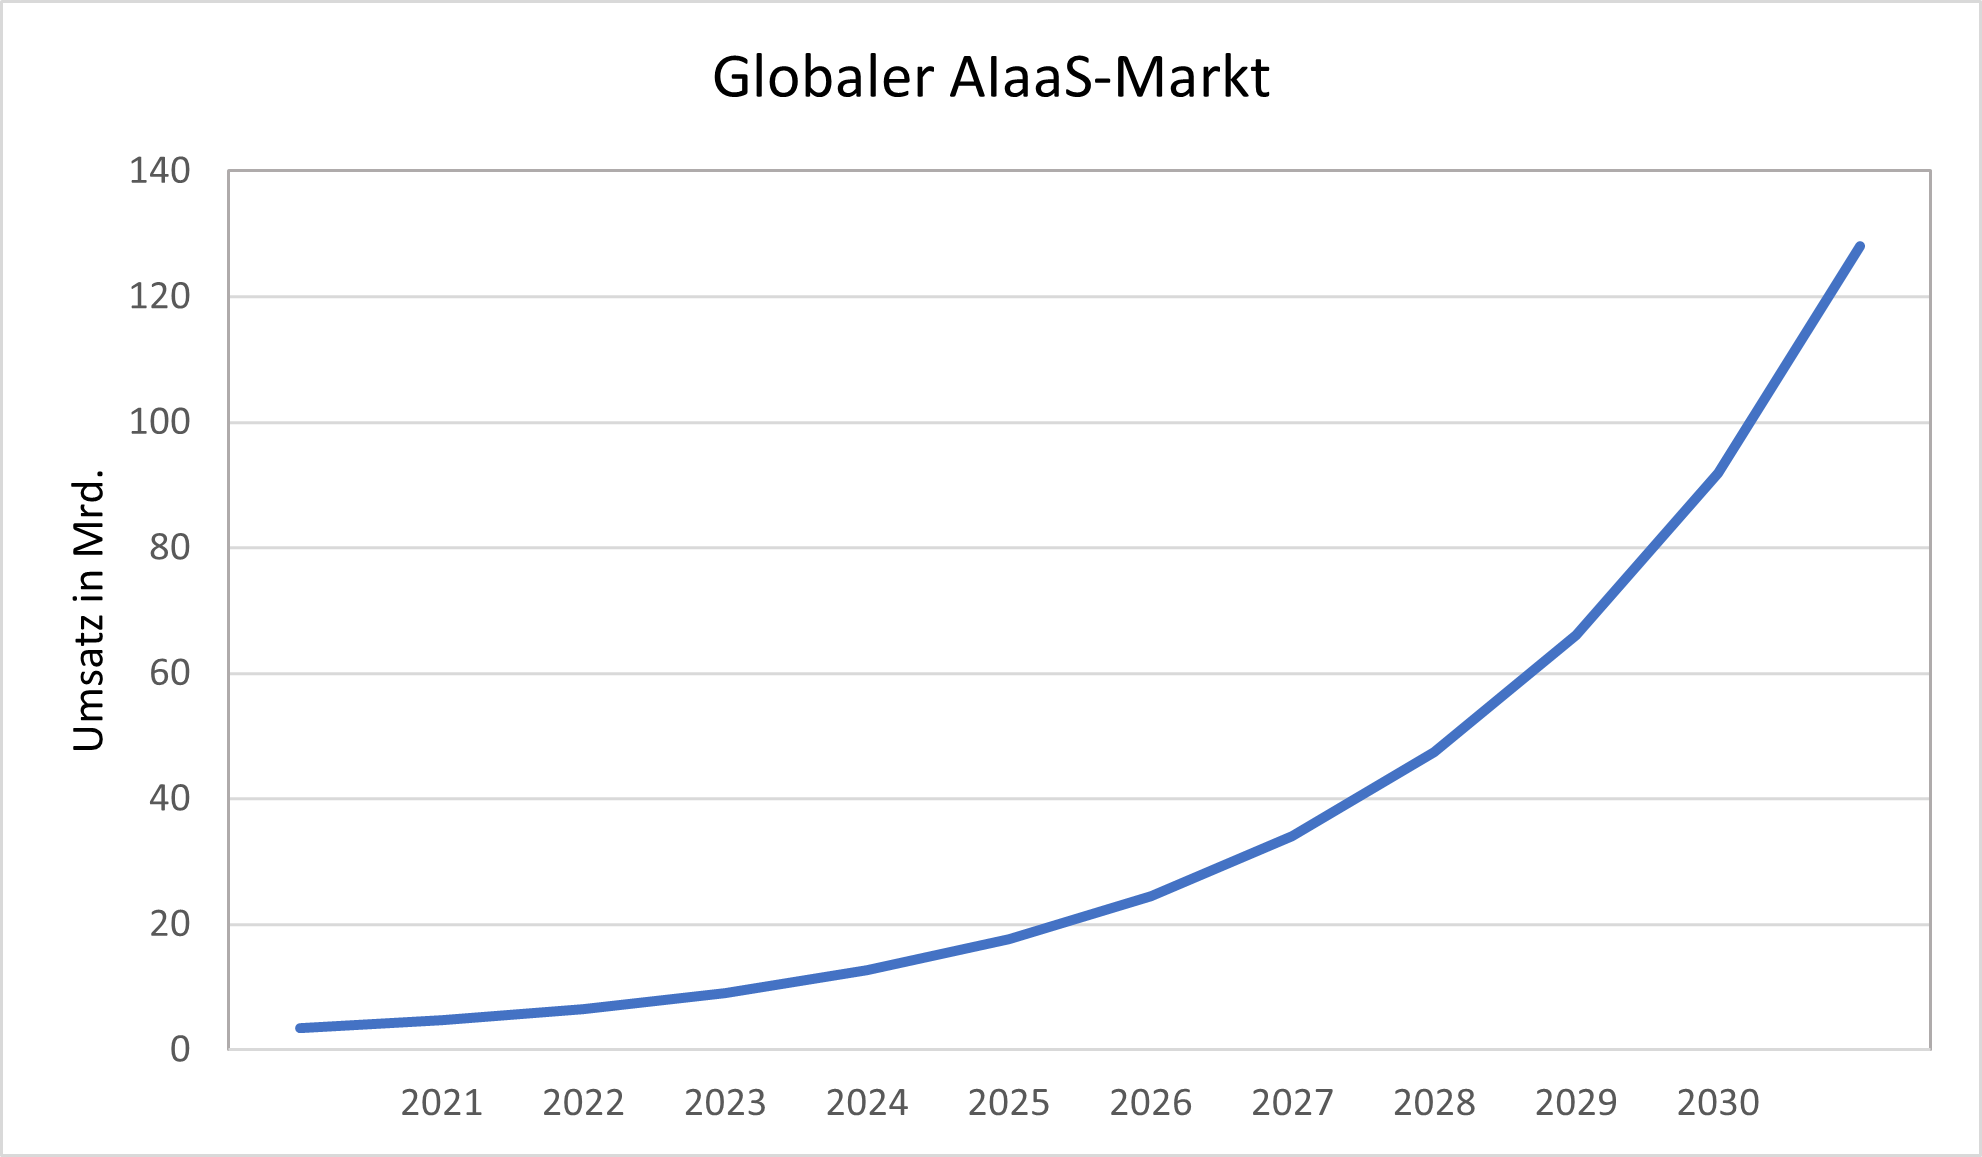
\includegraphics[width=\textwidth]{bilder/AIaaS-Markt.png}
  \caption{Prognostizierter, durchschnittlicher Marktverlauf bist 2030}
  \label{fig:aiaasmarkt}
\end{figure}


\subsection{Google LLC}
Google bietet eine Reihe von Diensten für künstliche Intelligenz an, mit denen Entwickler ihren Anwendungen problemlos intelligente Funktionen hinzufügen können. Zu diesen Diensten gehören vorab trainierte Modelle für maschinelles Lernen, die für Aufgaben wie Bilderkennung, Verarbeitung natürlicher Sprache und prädiktive Analysen verwendet werden können. Google bietet auch eine Cloudbasierte Entwicklungsumgebung für die Erstellung und das Training benutzerdefinierter maschineller Lernmodelle. Dieser Ansatz erleichtert Entwicklern den Einstieg in die KI, ohne dass sie in teure Hardware oder Software investieren müssen.
Zu den von Google angebotenen Produkten gehören unter anderem die Google Cloud Natural Language API, Cloud Speech API, Cloud Translation API und Cloud Vision API. Diese Dienste ermöglichen es Entwicklern, Anwendungen zu erstellen, die menschliche Sprache verstehen, Sprache in Text umwandeln, zwischen Sprachen übersetzen und Objekte in Bildern identifizieren können. Dabei können die Services mit einer simplen API-Anbindung in die eigenen Softwareprodukte eingebunden werden. \cite[vgl.][]{GoogleCloud.OA.2022}


\subsection{Microsoft Corporation}
Microsofts Ansatz für AIaaS bietet Entwicklern eine Reihe von Möglichkeiten, KI-Funktionen in ihre Anwendungen mit einzubinden. Dabei werden über eine cloudbasierte Plattform Bereiche wie die Bildverarbeitung, Sprachverarbeitung, Übersetzungen und Suchen bereitgestellt. Microsofts Ansatz für KI als Service zielt darauf ab, das Hinzufügen von KI-Fähigkeiten zu Anwendungen zu erleichtern, ohne dass dafür tiefgreifende KI-Kenntnisse erforderlich sind.  Das Unternehmen bietet auch eine Reihe von Tools und Ressourcen, die Entwickler für die Erstellung von KI-Anwendungen nutzen können, darunter zählt beispielsweise die Azure Machine Learning-Plattform.
Ein Key-Product von Microsoft im Bereich von Künstlicher Intelligenz als Service ist die Microsoft Azure Cognitive Services Suite. Diese stellt eine Reihe von APIs in den bereits genannten Gebieten: Bild- und Sprachverarbeitung, Übersetzungen und Suchen bereit, mit denen intelligente Funktionen durch einfache API-Anfragen in Anwendungen hinzugefügt werden können. Ein weiteres Produkt ist die Cortana Intelligence Suite. Diese umfasst intelligente Dienste zur Datenanalyse, zum maschinellen Lernen und zur Verarbeitung natürlicher Sprache. \cite[vgl.][]{Azure.OA.2022}

\newpage
\subsection{Amazon Web Services Inc.}
Amazons Ansatz der künstlichen Intelligenz als Service ist ein Cloud-basierter Dienst, der Entwicklern Tools zur Erstellung und Bereitstellung von KI-Anwendungen zur Verfügung stellt. Der Service bietet eine Vielzahl von Funktionen, darunter vortrainierte Modelle, eine benutzerfreundliche Oberfläche und Unterstützung für zahlreiche Programmiersprachen. Amazon bietet eine Reihe von KI-Diensten an, die es Entwicklern ermöglichen, anspruchsvolle Anwendungen mit Funktionen der künstlichen Intelligenz zu erstellen. Zu diesen Services gehören Amazon Lex, Amazon Polly, Amazon Rekognition und Amazon SageMaker. Amazon Lex ist ein Service, der es Entwicklern ermöglicht, Conversational Bots zu erstellen. Er nutzt die Verarbeitung natürlicher Sprache (NLP), um die Absichten der Benutzer zu verstehen und Benutzeranfragen zu erfüllen. Amazon Polly ist ein Text-to-Speech-Service, der Text in lebensechte Sprache umwandelt. Er unterstützt eine Reihe von Sprachen und kann verwendet werden, um Anwendungen zu erstellen, die sprechen. Das kann beispielsweise beim Erstellen einer Barrierefreien Software helfen. Amazon Recognition ist ein Bilderkennungsdienst, der zur Identifizierung von Objekten, Personen und Szenen in Bildern verwendet werden kann. \cite[vgl.][]{AWS.OA.2022}


\subsection{IBM Corporation}
Der IBM-Ansatz für künstliche Intelligenz als Service basiert auf der Watson-Plattform des Unternehmens. Neben der „klassischen“ Möglichkeit eigene KI-Modelle zu trainieren und sie dann in einer Cloud-Umgebung einzusetzen, umfasst die Plattform auch eine Reihe von APIs, die es Entwicklern ermöglicht, von ihren eigenen Anwendungen aus auf die Fähigkeiten von Watson zuzugreifen.
Einer der populärsten Bereiche, die die IBM Watson Services abdecken ist das maschinelle Lernen. Dabei wird Unternehmen die Möglichkeit geboten, automatisch aus Daten zu lernen und die eigenen Prozesse zu verbessern. Die Services nutzen eine Vielzahl von Algorithmen, um Unternehmen in die Lage zu versetzen, Vorhersagemodelle zu erstellen, die für eine Reihe von Aufgaben wie Betrugserkennung, Kundensegmentierung und vorausschauende Wartung verwendet werden können.
Ein weiteres wichtiges Segment ist die Verarbeitung natürlicher Sprache. Hier wird es zum einen ermöglicht, aus unstrukturierten Daten wie Text und Audio eine Bedeutung zu extrahieren. Es ist zum anderen aber auch möglich die Services für Stimmungsanalysen, Inhaltsklassifizierungen und Entitätsextraktion zu verwenden.
IBMs Lösungen für die Informationsextraktion aus Bildern nennt man IBM Computer Vision Services. Sie können für Aufgaben wie Objekterkennung, Bildklassifizierung und Bildsuche genutzt werden. \cite[vgl.][]{IBM.OA.2021} \\
\subsection{Preisvergleich}
Jeder Anbieter bietet verschiedene Preis- und Abrechnungsmodelle an und stellt verschiedene KI-Lösungen zur Verfügung. Ein eindeutiger Preisvergleich über alle Funktionen zwischen den verschiedenen Unternehmen ist daher nur begrenzt möglich. Um trotzdem einen direkten Vergleich zu erhalten, haben wir uns die Speech-to-Text-Lösungen der einzelnen Anbieter angeschaut. Diese wurde gewählt, da sie von allen Firmen angeboten wird und es sich hierbei um eine Standardlösung handelt, die in vielen Bereichen angewendet werden kann und kein „Nischenprodukt“, das speziell für eine Branche entwickelt wurde, ist. Bei Speech-to-Text wird gesprochene Sprache erkannt und in geschriebenen Text umgewandelt. Die Anwendungsgebiete dafür reichen von intelligenten persönlichen Assistenten wie Apples Siri oder Amazons Alexa, über das Mitschreiben und Dokumentieren von Meetings oder Interviews, bis hin zur barrierefreien Gestaltung von Softwareprodukten, um Menschen mit Behinderung einen leichteren Zugriff auf digitale Inhalte zu ermöglichen. Zusätzlich gibt es zum Teil Zusatzfunktionen, die das Gesprochene gleichzeitig noch übersetzen oder sogar den Sprechenden verifizieren oder identifizieren können. \\

Google bietet seinen Kunden eine kostenlose Nutzung der Speech-to-Text-API von 60 Audiominuten pro Monat. Für alles darüber hinaus berechnet Google pro 15 Sekunden mindestens 0,004 \$. Das sind 0,016 \$ pro Minute. Dabei wird jede Anfrage auf die nächsten vollen 15 Sekunden aufgerundet. Bestimmt wird der endgültige Preis durch weitere Faktoren wie die Spracherkennung mit einem erweiterten KI-Modell, dem aktivieren von Daten-Logging oder der Anzahl der erkannten Audiokanäle der Daten. Begrenzt ist die Nutzung der API auf 1.000.000 Audiominuten pro Monat. Möchte man mehr Sprache erkennen, muss man bei Google eine Kontingentanfrage einreichen und Google über seinen Bedarf aufklären. \cite[vgl.][]{GoogleCloud.PV.2022} \\ 
Amazon Transcribe bietet seinen Kunden ebenfalls 60 Freiminuten pro Monat, allerdings nur für ein Jahr. Spätestens danach muss man auch hier nach Audiominuten dafür bezahlen. Hierbei ist das Preismodell Stufenweise mit drei verschiedenen Tier-Stufen aufgebaut. Für die ersten 250.000 Minuten im Monat zahlt man 0,024 \$/Minute. Für die nächsten 750.000 0,015 \$/Minute und für jede weitere Minute über 1.000.000 0,0102 \$. \cite[vgl.][]{AWS.PV.2022} \\
Bei den Microsoft Speech Services erhalten Kunden in der kostenlosen Version pro Monat fünf Audiostunden umsonst. Um mehr Daten zu verarbeiten, bietet Microsoft diesen Service für einen Dollar pro Audiostunde an. Das entspricht etwa 0,0167 \$/Minute. Außerdem bietet Microsoft auch verschiedene „Commitment Tiers“ an. Darauf muss man sich bewerben und kann dann für einen fixen Preis eine fixe Anzahl an Audiostunden erwerben. So zahlt man für 2.000 Stunden 1.600 Dollar, für 10.000 Stunden 6.500 Dollar und für 50.000 Stunden 25.000 Dollar. \cite[vgl.][]{Azure.PV.2022} \\
Auch IBM mit dem Watson Speech-to-Text-Service bietet verschiedene Preispläne an. Mit dem „Lite“-Plan erhält man kostenlos pro Monat 500 Audiominuten. Mit dem „Plus“-Plan zahlt man bis zu 1.000.000 Minuten 0,02 Dollar pro Minute, alles darüber kostet dann nur noch die Hälfte, nämlich 0,01 Dollar pro Minute. Zusätzlich gibt es noch die Pläne „Premium“ und „Deploy Anywhere“. Diese bieten weitere Zusatzfunktionen, wie zum Beispiel eine zusätzliche Datenverschlüsselung. Die Preise dieser Pläne sind allerdings nur auf Nachfrage einsehbar. \cite[vgl.][]{IBM.PV.2021} \\

Die Tabelle (siehe \autoref{tab:preisvergleich}) fasst die Preise der Anbieter zusammen. \\

\begin{table}[]
\def\arraystretch{2}
\begin{tabular}{|l|l|l|l|}
\hline
          & kostenlos                        & Weiterführend                                                                                                                     & Begrenzung       \\ \hline
Google    & 60min/M                       & 0.016\$/min                                                                                                                      & 1.000.000min/M \\ \hline
Amazon    & 60min/M (1 Jahr lang)                & \begin{tabular}[c]{@{}l@{}}0.024\$/min(bis 250.000min)\\ 0,015\$/min(bis 1.000.000min)\\ 0.0102\$/min(danach)\end{tabular}          & keine            \\ \hline
Microsoft & 300min/M (kostenlose Version) & \begin{tabular}[c]{@{}l@{}}\textbf{Einfacher Gebrauch:} 0,0167\$/min\\ \textbf{Commitment Tiers:}\\ 1.600\$ für 2.000h\\ 6.500\$ für 10.000h\\ 25.000\$ für 50.000h\end{tabular} & keine            \\ \hline
IBM       & Lite-plan 500min/M             & \begin{tabular}[c]{@{}l@{}}0.02\$/min (für 1.000.000min)\\ 0.01\$/min (danach)\end{tabular}                                      & keine            \\ \hline
\end{tabular}
\caption{Preisvergleich}\label{tab:preisvergleich}
\end{table}
\section{Vor- und Nachteile von AIaaS}
\subsection{Vorteile}
AIaaS zu nutzen kann viele Vor- aber auch Nachteile mit sich bringen. \\ \\
Wird AIaaS in einem Unternehmen genutzt, können Risiken verhindert werden, die in Verbindung mit dem Entwickeln und Warten von eigenen KI-Infrastrukturen auftreten könnten. Beim Neuentwickeln eigener KI´s ist keine Sicherheit gegeben, dass diese von Anfang an wie gewünscht funktioniert. Die Entwicklung von KI´s kann sehr komplex werden und kann deshalb bei Unternehmen, die bisher eher geringe Berührungspunkten mit KI´s hatten zu Fehleinschätzungen führen. Ein weiteres Risiko wäre zum Beispiel der Kontrollverlust der KI. Wird unbedacht oder blind auf diese Systeme vertraut, kann die Unabhängigkeit und Entscheidungsfreiheit verloren werden. Mit Nutzung von AIaaS können Risiken wie diese zwar nicht ausgelöscht werden, jedoch ist dort ein Know-how vorhanden, welches man selbst möglicherweise nicht besitzt. \\
Ein bekannter Fall, bei dem sich eine Künstliche Intelligenz selbstständig machte, ist ein Forschungsprojekt aus dem Jahr 2016. Hier versuchten zwei Forscher aus dem Google Brain Team zwei Maschinen miteinander kommunizieren zu lassen. Die Aufgabe dabei war, das Die Maschinen namens Bob und Alice Nachrichten verschicken, die nur der Gegenüber entziffern kann. Dagegen arbeitete eine dritte Maschine Namens Eve, die versuchte die Nachrichten zu entziffern. Anfangs konnte Eve viele Nachrichten entziffern, jedoch lernte Bob schnell und nach etwa 15 000 Durchläufen hatte Eve keine Chancen mehr die Nachrichten immer korrekt zu entziffern. Bob und Alice hatten einen Verschlüsselungsalgorithmus gefunden, den nur die beiden entschlüsseln konnten. Selbst die Wissenschaftler des Google-Teams konnten die Nachrichten nicht mehr nachvollziehen, da sie vergessen hatten zu implementieren, das die Bots sich ausschließlich auf Englisch unterhalten sollten und mussten das Projekt vorerst abbrechen. \cite[vgl.][]{Zeit.2016} \cite[vgl.][]{giga.2017} \\ \\
%https://www.zeit.de/digital/datenschutz/2016-10/google-kuenstliche-intelligenz-erfindet-eigene-verschluesselung?utm_referrer=https%3A%2F%2Fwww.google.com%2F    
% https://www.wissenschaftsjahr.de/2019/das-wissenschaftsjahr/da-kommt-ja-kein-mensch-drauf/was-reden-die-denn-da-chatbots-geben-raetsel-auf/index.html
Außerdem kann durch das Nutzen von AIaaS Diensten den Unternehmen bei der Einhaltung von Datenschutz- und Sicherheitsvorschriften helfen, da diese mit den Regelungen und Vorschriften vertraut sein sollten. Falls personenbezogene Daten vom Dienstleister verarbeitet werden, muss der Nutzer einen Auftragsverarbeitungs-Vertrag schließen. Der abgeschlossene AV-Vertrag regelt die Rechte und Pflichten des Auftraggebers und Auftragnehmers sowie etwaiger eingesetzter Sub-Dienstleister. Es sollte sichergestellt werden, dass  Auftragnehmer die einem anvertrauten Daten nur für den Zweck verarbeitet werden, für den der Auftraggeber die Daten erhoben hat. Vor allem aber sind Dienstleister verpflichtet,  Daten in angemessenem Umfang zu schützen. Um dies in der Praxis sicherzustellen, gibt der Vertrag dem Kunden diesbezüglich umfassende Kontrollrechte. \cite[vgl.][]{ActiveMindAG.2022} \\ \\
%https://www.activemind.de/datenschutz/dokumente/av-vertrag/
Mit AIaaS können KI-Fähigkeiten schnell und effizient skaliert werden. Das bedeutet, dass bei hohem Gebrauch der Dienste, mehr Cloud-Speicher dazu gebucht werden kann. Das gleiche gilt auch für die andere Richtung. Werden weniger Kapazitäten benötigt, so kann die Nutzung herunter skaliert werden. Testet ein Unternehmen beispielsweise mehrere Anbieter, um zu sehen, welche am bestem geeignet für es ist, so werden geringere Kapazitäten benötigt, wie bei einer Vollauslastung auf ein anstehendes Projekt bei einem Anbieter. \cite[vgl.][]{Cuofano.2022} \\
Die Lufthansa Industry Solutions beschreiben die Skalierbarkeit ihrer Service mit folgendem Satz:\glqq AIaaS kann je nach Bedarf und Wachstum des Unternehmens nach oben oder unten skaliert werden. Sämtliche KI-Tools lassen sich einzeln hinzufügen, sodass Unternehmen auch mit kleinen Schritten den Weg zur Nutzung von künstlicher Intelligenz gehen können\grqq. \cite[vgl.][]{LIS.2022} \\ \\
%https://www.lufthansa-industry-solutions.com/de-de/loesungen-produkte/kuenstliche-intelligenz/ai-as-a-service-automatisierung-von-geschaeftsprozessen
Ein weiterer Vorteil für die Nutzung von AIaaS ist der Zugang zu den neuesten und fortschrittlichsten KI-Technologien für die Unternehmen. Anbieter von AIaaS müssen stets auf dem aktuellen Stand sein, um auf dem Markt kompetitiv zu bleiben. Dadurch kann als Verbraucher immer eine verlässliche und fortschrittliche Technik erworben werden. Im Vergleich zu einer eigenen Implementierung wird auch hier viel Zeit gespart. Es würde einige Zeit dauern, um qualitativ auf das Level der Anbieter in dem Gebiet zu kommen. \cite[vgl.][]{Folio.2022} \\ \\
Der wohl größte Vorteil, der sich durch AIaaS ergibt, sind die Kosteneinsparungen. Durch Nutzung einer KI-Dritter, werden die kompletten Kosten für Entwicklung und Wartung einer eigenen KI eingespart. Es müssen ebenfalls keine Mitarbeiterkosten dafür gezahlt werden. Ein weiterer Vorteil, der sich dadurch ergibt, ist dass man sich auf seine Kernkompetenzen konzentrieren und die Pflege der KI-Infrastruktur den Experten überlassen kann.\\
Zahlen der Lufthansa Industry Solutions ergeben, dass die Effektivität der Prozesse um 60\% gesteigert werden können und die damit einhergehende Zeitersparnis eine Kostensenkung von bis zu 20 Prozent zur Folge hat. Des weiteren wird ein Tool zur Verfügung gestellt, bei dem man seine Anfragen pro Monat, die Minuten zur Bearbeitung einer Anfrage und die Kosten pro Stunde angibt. Mit diesen Informationen lassen sich die aktuellen Kosten in etwa bestimmen und gleichzeitig lassen sich die Kosten bei Nutzung von AIaaS ansehen.
%https://www.lufthansa-industry-solutions.com/de-de/loesungen-produkte/kuenstliche-intelligenz/ai-as-a-service-automatisierung-von-geschaeftsprozessen 
%gleich wie oben valla
Somit kann sich der Kunde ein Bild davon machen, ob es sich lohnt, AIaas einzuführen oder nicht. \cite[vgl.][]{LIS.2022} \\ 

\subsection{Nachteile}
Es gibt demzufolge viele Vorteile, die AIaaS mit sich bringt. Jedoch gibt es auch einige Nachteile, weshalb AIaaS nicht die perfekte Lösung darsellen könnte:\\
Es besteht immer die Gefahr, dass KI als Dienstleistung zur Entwicklung von autonomen Waffen oder anderen gefährlichen Technologien genutzt werden könnte. Auch wenn der Fall eher unwahrscheinlich ist, muss dieser beachtet werden. Der Nutzer muss nicht einmal unbedingt etwas böses im Sinn haben. Es reicht aus, wenn durch Fehler die künstliche Intelligenz intelligenter als der Mensch wird. Dadurch wird die KI unkontrollierbar und unvorhersehbar und es entstehen potenzielle Bedrohungen für die Welt und unsere Spezies. \\
In der 42. Deutschen Konferenz über Künstliche Intelligenz ging es unter anderem um KI-Systeme für das Militär. KI-Systeme werden sowohl für autonome Waffensysteme, als auch zur Lagebeurteilung benutzt. Damit soll frühzeitig erkannt werden, ob beispielsweise ein feindlicher Raketenangriff droht. Somit kann ein menschlicher Entscheidungsträger schnell Vergeltungsschläge ausführen. Laut Experten könnten solche KI's zur Destabilisierung der internationalen Beziehungen führen und auch zu Konflikten, die sich verselbstständigen. Viele Länder möchten ein Verbot autonomer Waffen. Jedoch lehnen große Waffenhersteller wie Russland, die USA und Israel die Forderungen ab. \cite[vgl.][]{Deutschlandfunk.2019}

%https://www.deutschlandfunk.de/autonome-waffen-ki-systeme-im-militaer-100.html
Der Einsatz von AIaaS könnte zu Arbeitsplatzverlusten und anderen wirtschaftlichen Störungen führen. Logischerweise folgt aus den Kosteneinsparungen bei Nutzung von KI´s ein geringeres Personal, das benötigt wird. Setzen sich Dienstleistungen und KI´s in einem größerem Feld durch, können viele Arbeiter ihren Arbeitsplatz dadurch verlieren. Das kann wiederum zu wirtschaftlichen Störungen auf dem Markt führen.

Ein anderer Punkt ist, dass AIaas das Risiko von Cyberangriffen und anderen bösartigen Aktivitäten erhöhen könnte. Durch die einfache Möglichkeit, an qualitativ hochwertige KI´s zu kommen, können Menschen mit boshaften Absichten diese KI´s ausnutzen, um Leute oder gar Firmen mit Cyberangriffen zu drohen oder gar durchzuführen.

Letzten Endes muss noch angesprochen werden, dass AIaaS genutzt werden kann, um Nutzer auszubeuten und zu manipulieren sowie ihre Privatsphäre zu verletzen. KI´s sind sehr modern und viel gefragt. Dadurch kann ein potenzieller Nutzer sehr einfach manipuliert werden, sehr hohe Preise für eine kleine KI zu zahlen. Außerdem kann die Privatsphäre von Kunden sehr schnell angegriffen werden. Zum Lernen benötigt die KI meist sehr viele Daten. Oft werden dafür auch Daten von Kunden genommen, die normalerweise einen privaten Status haben. \cite[vgl.][]{InApp.2020}

Ein aktueller Fall zeigt, dass das Einsetzen und zur Verfügung stellen von einem KI-Tool auch rechtliche Konsequenzen für den Anbieter haben kann, welcher die Schäden aber auch an seine Kunden weitergeben könnte. Eine aktuelle Sammelklage richtet sich gegen die Unternehmen GitHub, den Mutterkonzern Microsoft und das KI-Unternehmen OpenAI. Die von GitHub angeboten Programmierhilfe mit dem Namen GitHub Copilot soll laut Klage keine Quellen angeben, woher der generierte Code kommt, der zur Verfügung gestellt wird. Dadurch werden die Open-Source-Lizenzmodelle und die Rechte der Programmierer des Codes verletzt. \\
Copilot ist seit Juni 2022 zugänglich und bietet dem Nutzer Vorschläge, wie der momentane Code vervollständigt werden kann. Das KI-System greift dabei auf viele öffentliche Code-Repositorys in GitHub zurück. Dabei wird der Ersteller es Codes jedoch nicht um Erlaubnis gefragt. Die Klage beschreibt einen Verstoß gegen die Richtlinien des Digital Millennium Copyright Act (DMCA). Laut Klage verstößt die Software drei Mal gegen Abschnitt 1202 DMCA – fehlender Verweis aufs Urheberrecht, fehlende Namensnennung, sowie fehlender Lizenztext. Würde man davon ausgehen, dass jeder Copilot Nutzer einmal gegen den Abschnitt 1202 verstoßen hat, so würden sich 3.600.000 Verstöße durch GitHub ansammeln. Der Mindestschadenersatz läge dabei bei 2500 US-Dollar pro Einzelfall. Somit kommt man auf eine Gesamtsumme von 9 Milliarden Dollar. Dazu kommen noch weitere in der Klageschrift vorgeworfene Rechtsverstöße wie unlauterer Wettbewerb oder der Verstoß gegen das kalifornische Verbraucherschutzgesetz. \cite[vgl.][]{Wittenhorst.2022}  \\
\newpage
\section{Fazit}
\subsection{Argumentationsfazit}
Zusammenfassend lässt sich also sagen, dass es durchaus Zahlreiche Argumente gibt, die für den Einsatz von AIaaS im Unternehmensumfeld sprechen. Allerdings gibt es auch einige Gegenargumente die potenziell auftretende Probleme und Gefahren beschreiben. Hierbei gilt, dass jedes Unternehmen für sich erörtern und entscheiden muss wie mit diesen Punkten umgegangen wird und ob man die eventuellen Sicherheitslücken mit eigenen Ressourcen und Know-How schließen kann. \\
Man kann hier also deutlich sehen, dass, auch wenn das so von den verschiedenen Service Providern vermarktet und angepriesen wird, es nicht möglich, bzw. nicht empfehlenswert ist, einfach eine vorhandene künstliche Intelligenz in seine Systeme einzubinden. Man muss zahlreiche Modifikationen vornehmen. Allerdings: Hat man einmal initial die erforderlichen Anpassungen vorgenommen, hat man in der Regel weniger Wartungsaufwand als bei einer hauseigenen on-premise-Lösung, da das weitere Trainieren der KI und auch weitere Optimierungen bezüglich der Sicherheit oder Performance von den Providern durchgeführt wird. \\

\subsection{Anbieterfazit}
Wenn man sich für einen AIaaS-Dienst entschieden hat, geht es bei der Anbieterwahl primär darum, welcher von ihnen eine Lösung anbietet, die für mein Produkt geeignet ist. Viel Provider bieten eine Vielzahl an Diensten an, welche sich nur wenig unterscheiden. Neben den oben genannten Hauptakteuren am Markt kann man sich natürlich auch für einen kleineren Anbieter entscheiden. Das bietet den Vorteil, dass man eventuell einen größeren Verhandlungsspielraum hat, wenn es um Anfragen zu Zusatzfunktionen oder Anpassungen des KI-Modells geht. Bei großen Firmen wie Google oder Amazon hat man bei solchen Anfragen meist keinen Erfolg, da die Produkte für die breite Masse konzipiert sind und Individualanpassungen eher unüblich sind. Was jedoch ein großer Vorteil bei den ,,Big Playern`` ist, ist dass sie schon ein globales Netz an Rechenzentren zur Verfügung haben und somit eine hohe Ausfallsicherheit gewährleistet ist. Außerdem ist bei diesen Anbietern garantiert, dass die KI-Services kontinuierlich gewartet, erweitert und verbessert werden, da es dedizierte Teams dafür gibt.

\newpage
\subsection{Zukunftsaussicht}
Die Zukunft von Everything-as-a-Service sieht sehr vielversprechend aus. Getrieben wird das Wachstum von XaaS durch die Kombination aus der hohen Nachfrage an Cloud Computing und der wachsenden Infrastruktur des globalem Internets mit einer hohen Bandbreite. Im Zuge diesen technologischen Fortschritts nutzen Unternehmen vor allem immer mehr Software-as-a-Service-Lösungen (SaaS) für ihren Betrieb. Es ist zu erwarten, dass sich in Zukunft immer mehr Unternehmen für dieses Modell entscheiden werden, das es ihnen ermöglicht, schnell und einfach auf die von ihnen benötigten Dienste zuzugreifen, ohne in teure Hardware und Software investieren zu müssen. Da Cloud Computing immer beliebter wird, werden auch die Kosten für XaaS-Lösungen immer attraktiver für Unternehmen aller Größenordnungen.

Der globale XaaS-Markt wurde 2021 von,,Allied Market Research`` auf etwa 474,9 Milliarden US-Dollar bemessen. Voraussichtlich wird der Markt 2031 auf bis zu 2,63 Billionen US-Dollar anwachsen. Das wäre eine Durchschnittliche jährliche Wachstumsrate von 18,9 Prozent. Dabei gibt es vor allem starke Nachfragen bei SaaS, aber auch bei IaaS und PaaS. Hauptsächliche Treiber des Wachstums sind hierbei Regierungen, die Gesundheitsindustrie und die produzierende Industrie.

Der Artificial-Intelligence-as-a-Service-Markt für sich wird zwar im vergleich zum allgemeinen XaaS-Markt voraussichtlich prozentual deutlich stärker anwachsen, wird jedoch trotzdem nur einen kleinen Teil des Gesamtmarktes ausmachen. Die Nachfrage an den klassischen Hauptkomponenten ist aktuell noch sehr hoch und und die Anwendungsgebiete für AIaaS, vor allem in kleinen bis mittleren Unternehmen, noch nicht sehr ausgereift. Viele Unternehmen werden sich in Zukunft wohl zunächst auf die reine Digitalisierung bzw. der digitalen Abbildung von Geschäftsprozessen fokusieren, um dann danach Ansätze zu Prozessoptimierung mittels künstlicher Intelligenz zu verfolgen. \cite[vgl.][]{AlliedMarketResearch.2022} \\

%%% Angabe der .bib-Datei (ohne Endung) / State .bib file (for BibTeX usage)

% If you want to break on URL numbers
\setcounter{biburlnumpenalty}{9000}
% If you want to break on URL lower case letters
\setcounter{biburllcpenalty}{9000}
% If you want to break on URL UPPER CASE letters
\setcounter{biburlucpenalty}{9000}

\newpage
\section{Literatur}
\printbibliography[title=""]
\end{document}
